\chapter{Soluția propusă}
\label{cap:cap3}

Acest capitol detaliază procesul de proiectare și implementare a platformei de găzduire VPS. Sunt prezentate cerințele sistemului, arhitectura generală, tiparele de proiectare adoptate, deciziile tehnologice, schema bazei de date și modul în care componentele software interacționează pentru a oferi o experiență de utilizare simplificată peste infrastructura OpenStack.

\section{Reiterarea problemei și strategia de rezolvare}
\label{sec:cap3_problema}

Interfețele native ale infrastructurilor cloud private (precum OpenStack Horizon) sunt proiectate pentru administrarea rețelelor complexe, nu pentru utilizatorii finali. Provocarea principală constă în abstractizarea acestei complexități fără a sacrifica controlul asupra resurselor.

Strategia de rezolvare propusă în această lucrare presupune dezvoltarea unui nivel intermediar (\textit{middleware}) care interceptează cererile simplificate ale utilizatorilor și le traduce automat într-o secvență de comenzi complexe către API-urile OpenStack: rezolvarea rețelei și a portului, instanțierea mașinii, alocarea unei adrese IP publice și atașarea volumelor de stocare.

La baza întregii soluții e un principiu de proiectare fundamental, care guvernează separarea responsabilităților: \textbf{nivelul API operează exclusiv asupra propriilor baze de date și nu apelează niciodată direct, în mod sincron, infrastructura OpenStack}; toate interacțiunile cu infrastructura sunt delegate unor procese de fundal. Acest principiu, detaliat în Secțiunea~\ref{sec:cap3_arhitectura}, asigură atât receptivitatea interfeței, cât și reziliența sistemului.

\section{Cerințele sistemului și ale utilizatorului}
\label{sec:cap3_cerinte}

Pentru a ghida procesul de dezvoltare, au fost definite o serie de cerințe clare, împărțite în cerințe funcționale (grupate pe domenii) și cerințe nefuncționale.

\subsection{Cerințe funcționale}

\textbf{Autentificare și model multi-tenant:}
\begin{itemize}
    \item \textbf{CF1:} Sistemul trebuie să permită înregistrarea, prin care se creează o organizație și un cont de utilizator-proprietar asociat, precum și autentificarea pe baza adresei de email și a parolei.
    \item \textbf{CF2:} Platforma trebuie să organizeze utilizatorii în organizații izolate logic, fiecare resursă fiind vizibilă exclusiv membrilor organizației proprietare.
    \item \textbf{CF3:} Sistemul trebuie să implementeze un control al accesului bazat pe roluri (proprietar, membru și administrator de platformă), restricționând operațiunile sensibile (ștergere, eliberare de resurse) la rolurile autorizate.
\end{itemize}

\textbf{Gestiunea instanțelor:}
\begin{itemize}
    \item \textbf{CF4:} Utilizatorul trebuie să poată vizualiza lista mașinilor virtuale ale organizației, cu starea acestora (\texttt{BUILD}, \texttt{ACTIVE}, \texttt{SHUTOFF}, \texttt{ERROR}) și adresele IP alocate.
    \item \textbf{CF5:} Utilizatorul trebuie să poată lansa una sau mai multe instanțe completând un formular cu numele, imaginea sistemului de operare, pachetul hardware (\textit{flavor}), cheia SSH și grupul de securitate.
    \item \textbf{CF6:} Utilizatorul trebuie să poată controla ciclul de viață al unei instanțe: pornire, oprire, repornire și ștergere.
    \item \textbf{CF7:} Sistemul trebuie să permită capturarea stării unei instanțe sub forma unei imagini reutilizabile (\textit{snapshot}).
    \item \textbf{CF8:} Utilizatorul trebuie să poată accesa o consolă interactivă (NoVNC) direct din browser și să poată consulta jurnalul de sistem (\textit{console log}) și jurnalul de evenimente al fiecărei instanțe.
    \item \textbf{CF9:} Sistemul trebuie să ofere șabloane preconfigurate (de exemplu, un server cu o aplicație preinstalată), realizate prin injectarea unui script de inițializare \textit{Cloud-init}.
\end{itemize}

\textbf{Rețea și stocare:}
\begin{itemize}
    \item \textbf{CF10:} Platforma trebuie să automatizeze provizionarea rețelelor private, a subrețelelor, a ruterelor și a grupurilor de securitate.
    \item \textbf{CF11:} Utilizatorul trebuie să poată gestiona adrese IP publice (\textit{floating IPs}) ca resurse de sine stătătoare: alocare, asociere, disociere și eliberare.
    \item \textbf{CF12:} Utilizatorul trebuie să poată crea, atașa, detașa și șterge volume de stocare bloc (Cinder), precum și să importe imagini de sistem personalizate de la un URL.
\end{itemize}

\textbf{Administrare și monitorizare:}
\begin{itemize}
    \item \textbf{CF13:} Administratorul de platformă trebuie să dispună de o consolă transversală, care oferă vizibilitate asupra tuturor organizațiilor și utilizatorilor și asupra capacității reale a cluster-ului OpenStack.
    \item \textbf{CF14:} Sistemul trebuie să aplice cote (\textit{quotas}) configurabile per organizație, respinse la depășire.
    \item \textbf{CF15:} Platforma trebuie să monitorizeze și să afișeze consumul de resurse (CPU) al instanțelor sub formă de grafice istorice.
\end{itemize}

Relațiile dintre actorii sistemului și principalele cazuri de utilizare sunt prezentate în diagrama cazurilor de utilizare, prezentată în Anexa~\ref{anexa:usecase}. Sistemul definește trei roluri, aflate într-o relație de specializare. \textbf{Membrul} reprezintă actorul de bază, cu acces la operațiile obișnuite de utilizare: autentificarea, crearea și vizualizarea instanțelor, controlul ciclului de viață (pornire, oprire, repornire), captura de imagini (\textit{snapshot}), gestiunea resurselor de rețea și de stocare, precum și accesul la consolă și la jurnale. \textbf{Proprietarul} moștenește toate cazurile de utilizare ale membrului și adaugă acțiunile sensibile, rezervate organizației: ștergerea instanțelor, eliberarea resurselor publice (adrese IP) și gestiunea echipei și a rolurilor. \textbf{Administratorul} este un actor de nivel platformă, situat deasupra organizațiilor, responsabil de configurarea cotelor și de administrarea globală a sistemului. Această ierarhie de actori se reflectă direct în modelul de control al accesului bazat pe roluri (RBAC), detaliat în secțiunea~\ref{sec:cap3_securitate}.

\subsection{Cerințe nefuncționale}
\begin{itemize}
    \item \textbf{Performanță și receptivitate:} Interfața web nu trebuie să se blocheze în timpul operațiunilor de lungă durată; cererile de modificare a infrastructurii trebuie confirmate într-un timp constant, indiferent de durata reală a provizionării.
    \item \textbf{Scalabilitate:} Componenta de backend trebuie să poată prelua cereri concurente, iar numărul de procese de fundal trebuie să poată fi mărit independent de serverul web.
    \item \textbf{Securitate:} Token-urile de sesiune nu trebuie să fie accesibile codului JavaScript, parolele trebuie stocate exclusiv sub formă de amprente criptografice, iar accesul la resurse trebuie izolat la nivel de organizație.
    \item \textbf{Reziliență:} O eroare tranzitorie a infrastructurii nu trebuie să compromită starea sistemului; operațiunile eșuate trebuie reîncercate automat, iar starea afișată trebuie reconciliată periodic cu starea reală a infrastructurii.
    \item \textbf{Utilizabilitate:} Interfața trebuie să ofere o experiență comparabilă cu cea a platformelor comerciale axate pe simplitate (DigitalOcean), ascunzând terminologia de administrare de infrastructură.
\end{itemize}

\section{Alegerea tehnologiilor și justificarea acestora}
\label{sec:cap3_tehnologii}

Platforma a fost dezvoltată folosind o stivă tehnologică modernă, aleasă pe criterii de performanță, suport pentru operațiuni asincrone și mentenabilitate.

\begin{itemize}
    \item \textbf{Frontend --- Nuxt (Vue.js) și Tailwind CSS:} Interfața este o aplicație de tip SPA (\textit{Single-Page Application}), construită cu framework-ul Vue.js, organizat prin meta-framework-ul Nuxt. Această abordare a fost preferată întrucât aplicația este un panou de administrare destinat utilizatorilor autentificați, pentru care indexarea de către motoarele de căutare este irelevantă, iar randarea pe partea de client simplifică semnificativ gestiunea sesiunilor bazate pe cookie-uri \textit{httpOnly}. Stilizarea Tailwind CSS a permis dezvoltarea rapidă a unei interfețe consistente.
    \item \textbf{Backend --- FastAPI (Python):} A fost preferat în detrimentul unor framework-uri clasice precum Django sau Flask datorită performanței sale ridicate și a suportului nativ pentru standardul ASGI (\textit{Asynchronous Server Gateway Interface}). FastAPI permite validarea automată a datelor prin biblioteca Pydantic și generarea automată a documentației (OpenAPI / Swagger UI).
    \item \textbf{Mesagerie și procesare asincronă --- RabbitMQ și Celery:} Pentru a respecta cerința de neblocare a interfeței, sarcinile costisitoare sunt transmise prin protocolul AMQP către \textbf{RabbitMQ}, un broker de mesaje robust care garantează livrarea. \textbf{Celery} a fost ales ca sistem de procese de fundal datorită mecanismelor avansate de reluare a sarcinilor (\textit{retries}) și a integrării naturale cu RabbitMQ.
    \item \textbf{Persistența datelor --- MariaDB, InfluxDB:} MariaDB asigură persistența datelor tranzacționale (utilizatori, organizații, instanțe, rețele), respectând proprietățile ACID. InfluxDB, o bază de date de tip \textit{Time-Series}, este utilizată strict pentru telemetrie, fiind optimizată pentru ingestia rapidă a metricilor marcate temporal.
    \item \textbf{Acces la infrastructură --- OpenStack SDK:} Comunicarea cu serviciile OpenStack se realizează prin biblioteca oficială OpenStack SDK, care abstractizează autentificarea și apelurile REST către componentele Nova, Neutron, Glance, Cinder și Keystone.
\end{itemize}

\section{Arhitectura generală a sistemului}
\label{sec:cap3_arhitectura}

Sistemul implementat urmează o arhitectură stratificată și orientată pe evenimente, asigurând o decuplare strictă între interfață, logica de dirijare a cererilor și logica de execuție efectivă a operațiunilor de infrastructură. Componentele majore și fluxul de comunicare sunt ilustrate în Figura~\ref{fig:arhitectura_detaliata}.

\begin{figure}[H]
    \centering
    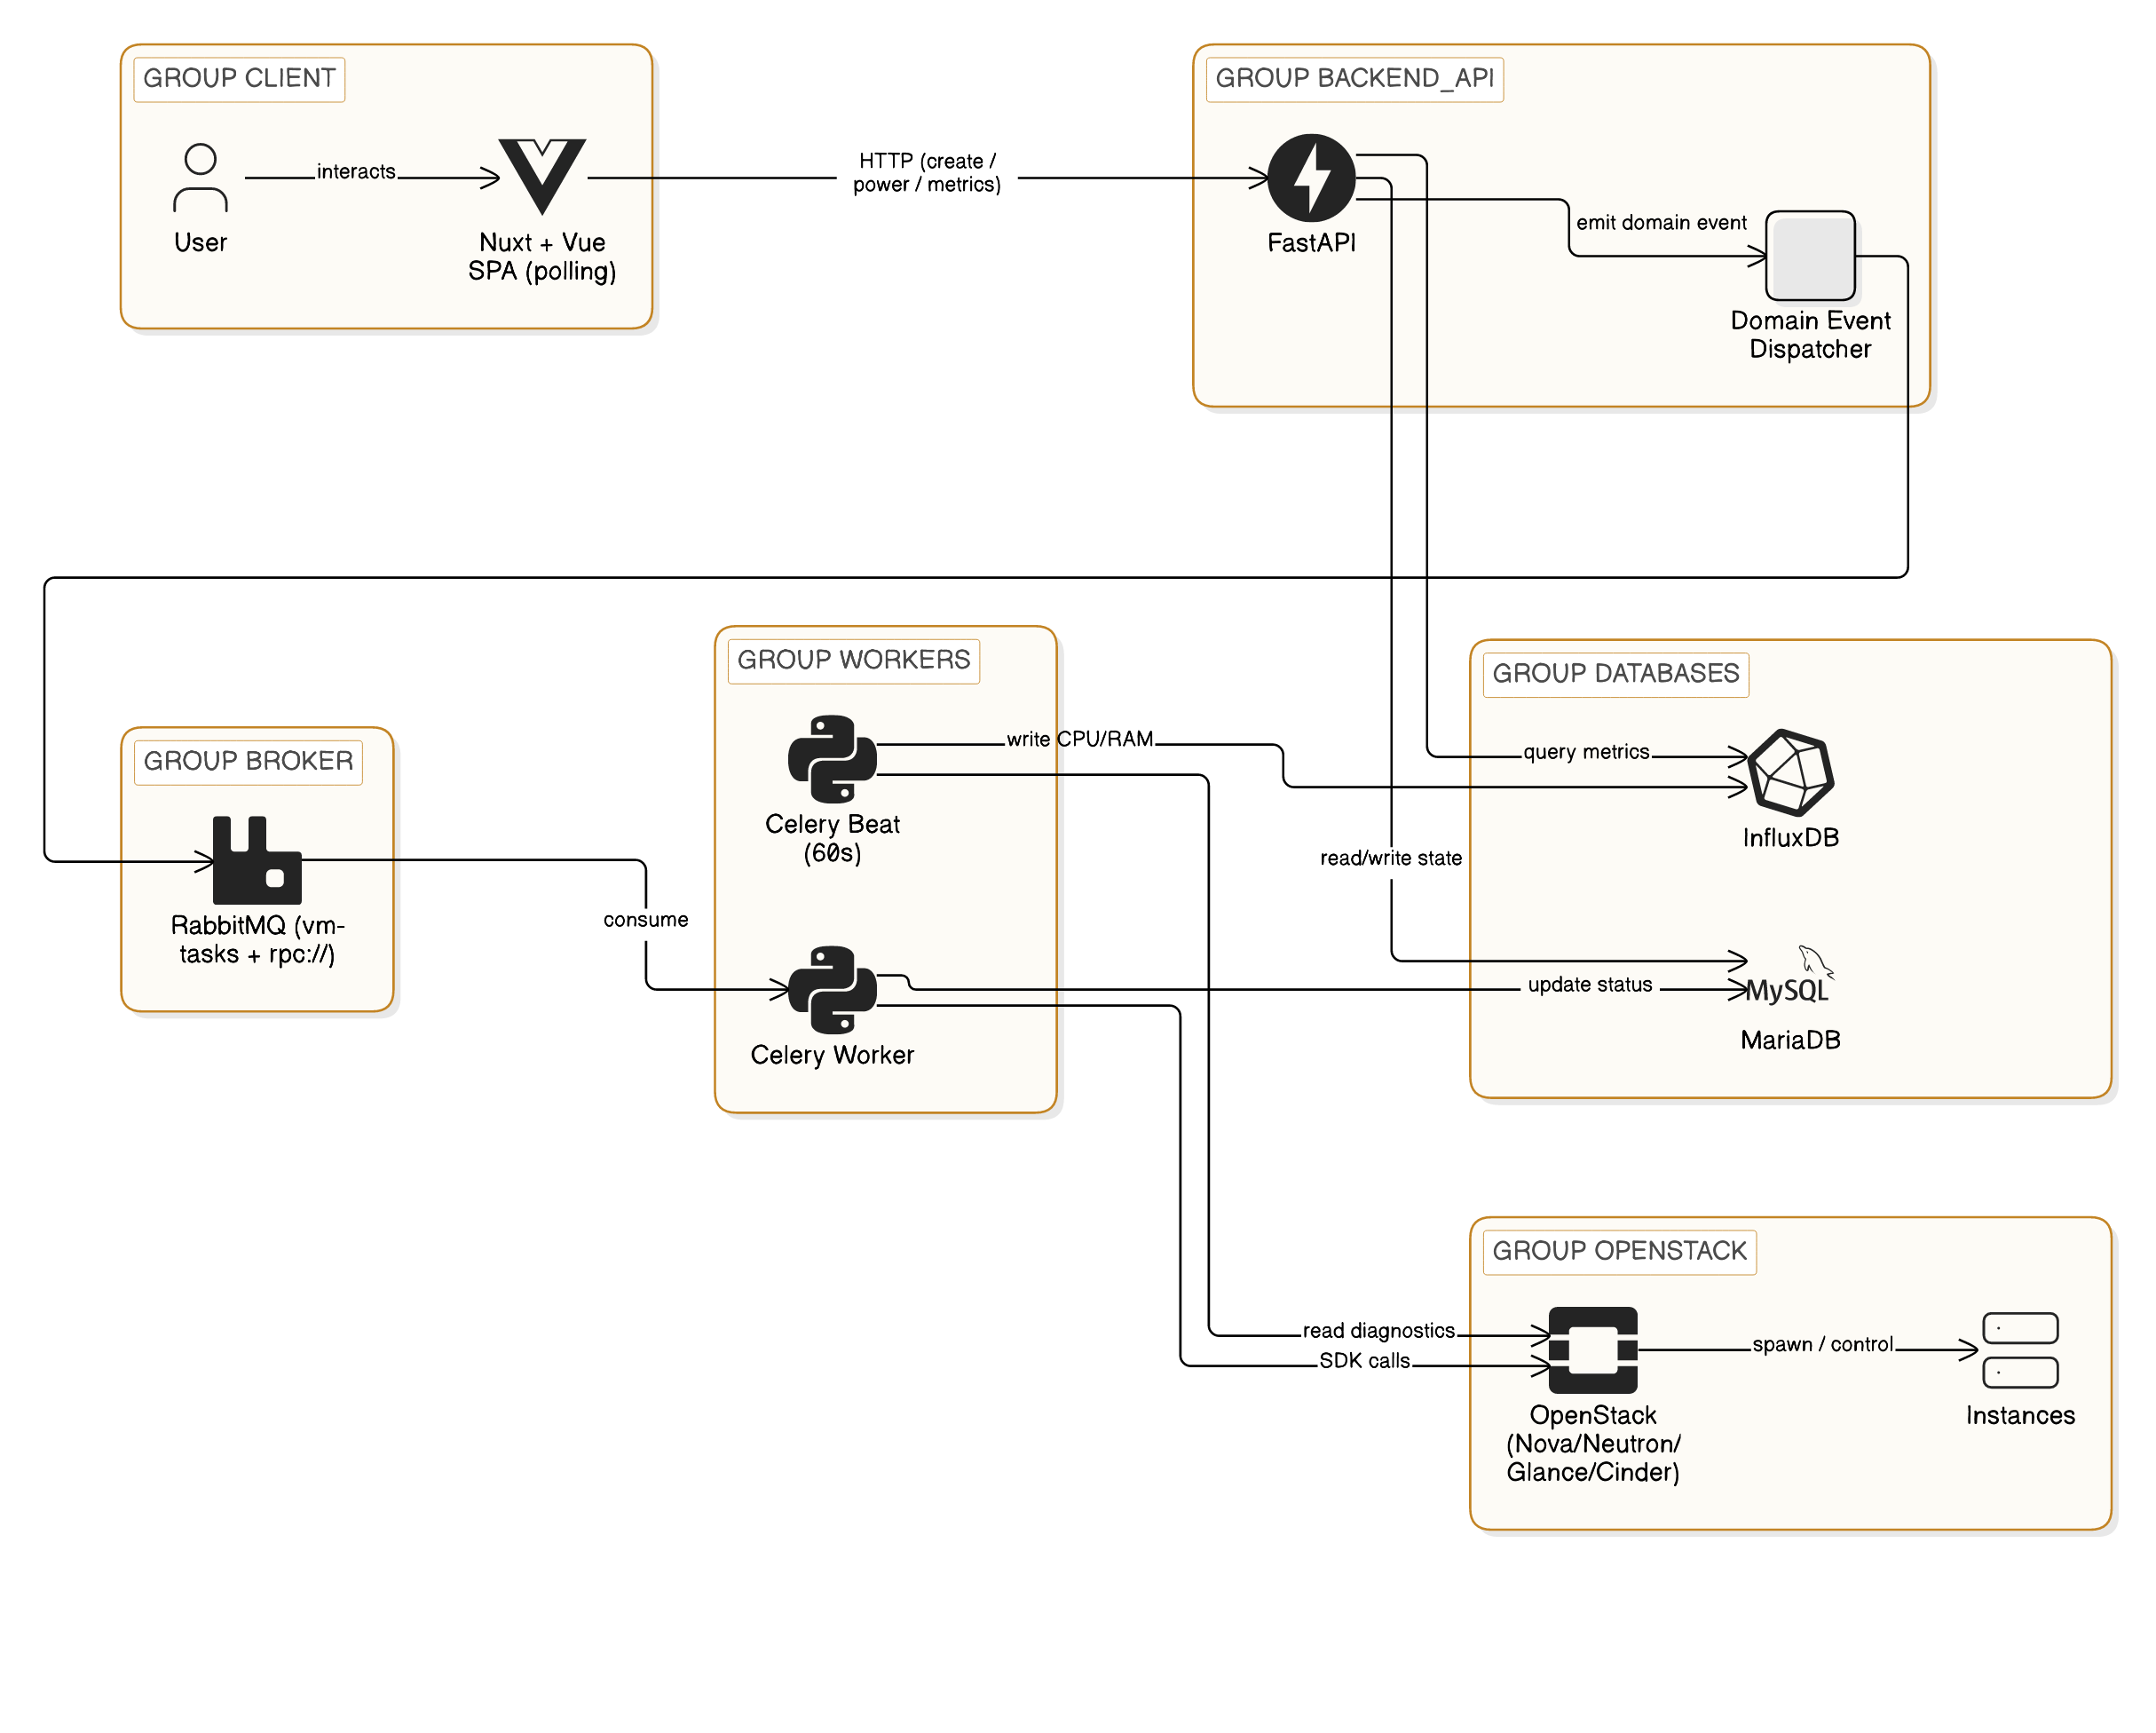
\includegraphics[width=\textwidth]{continut/capitol3/figuri/full_architecture.png}
    \caption{Arhitectura detaliată a sistemului, ilustrând fluxul asincron și componentele backend.}
    \label{fig:arhitectura_detaliata}
\end{figure}

Figura~\ref{fig:arhitectura_detaliata} grupează componentele în zone logice distincte, evidențiind faptul că singura cale dintre nivelul API și infrastructură trece prin broker-ul de mesaje, cele două nu sunt niciodată cuplate direct:

\begin{itemize}
    \item \textbf{Zona client} --- utilizatorul interacționează cu o aplicație de tip \textit{Single-Page Application} (Nuxt + Vue) care comunică cu serverul exclusiv prin cereri HTTP REST și obține actualizările de stare prin interogare periodică (\textit{polling}), fără conexiuni persistente.
    \item \textbf{Nivelul API (FastAPI)} --- primește cererile, le validează, persistă starea inițială a resursei și emite un eveniment de domeniu către dispecer (\textit{Domain Event Dispatcher}), răspunzând clientului imediat, fără a aștepta infrastructura.
    \item \textbf{Broker-ul de mesaje (RabbitMQ)} --- primește sarcinile puse în coadă de către dispecer și le livrează proceselor de fundal; servește totodată ca \textit{backend} de rezultate (\textit{rpc://}) pentru puținele apeluri sincrone, precum obținerea adresei consolei noVNC sau a jurnalelor.
    \item \textbf{Procesele de fundal (Celery)} --- workerul consumă sarcinile din broker și execută efectiv operațiunile, în timp ce planificatorul (\textit{Celery Beat}) declanșează periodic, la fiecare 60 de secunde, colectarea telemetriei și reconcilierea stărilor. Acestea sunt singurele componente care apelează direct OpenStack SDK.
    \item \textbf{Infrastructura OpenStack} --- serviciile Nova, Neutron, Glance și Cinder materializează mașinile virtuale, rețelele și volumele; workerul citește din ele atât rezultatul operațiunilor, cât și datele de diagnostic pentru telemetrie.
    \item \textbf{Bazele de date} --- MariaDB păstrează starea relațională (actualizată de worker după finalizarea operațiunii în infrastructură), iar InfluxDB stochează seriile de timp ale telemetriei; nivelul API citește din ambele pentru a servi clientul.
\end{itemize}

\subsection{Principiile fundamentale de proiectare}
\label{subsec:cap3_principii}

Întreaga arhitectură este guvernată de un set de reguli de proiectare care delimitează responsabilitățile componentelor și care reprezintă o contribuție centrală a soluției:

\begin{enumerate}
    \item \textbf{API-ul efectuează doar operațiuni de citire/scriere asupra bazelor de date proprii} (MariaDB și InfluxDB) și nu apelează niciodată direct biblioteca OpenStack SDK. Astfel, un eveniment de tip ștergere de instanță nu așteaptă răspunsul infrastructurii.
    \item \textbf{Procesele de fundal (Celery) dețin exclusiv toate apelurile către OpenStack SDK.} Crearea mașinilor virtuale, provizionarea rețelelor sau colectarea telemetriei sunt realizate integral de către procesele de fundal.
    \item \textbf{Evenimentele de domeniu (\textit{Domain Events}) decuplează serviciile de procesarea asincronă.} Serviciile emit evenimente printr-un dispecer (\textit{dispatcher}), iar procesele de fundal înregistrează gestionari (\textit{handlers}) pentru aceste evenimente. Serviciile nu au cunoștință despre existența Celery.
    \item \textbf{Rețelistica este de tip VPC.} Nu există rețele globale predefinite; fiecare organizație dispune de rețele private proprii, iar adresele IP publice provin dintr-un bazin extern.
\end{enumerate}

Aceste reguli explică modul în care erorile fizice ale infrastructurii (de exemplu, lipsa capacității de calcul) nu se manifestă ca erori HTTP sincrone, ci sunt reconciliate ulterior în baza de date și reflectate prin starea resursei.

\subsection{Fluxul asincron de provizionare}
\label{subsec:cap3_flux}

Fluxul complet de creare a unei instanțe, de la cererea utilizatorului până la materializarea mașinii virtuale, este prezentat în diagrama de secvență din Figura~\ref{fig:secventa}.

\begin{figure}[H]
    \centering
    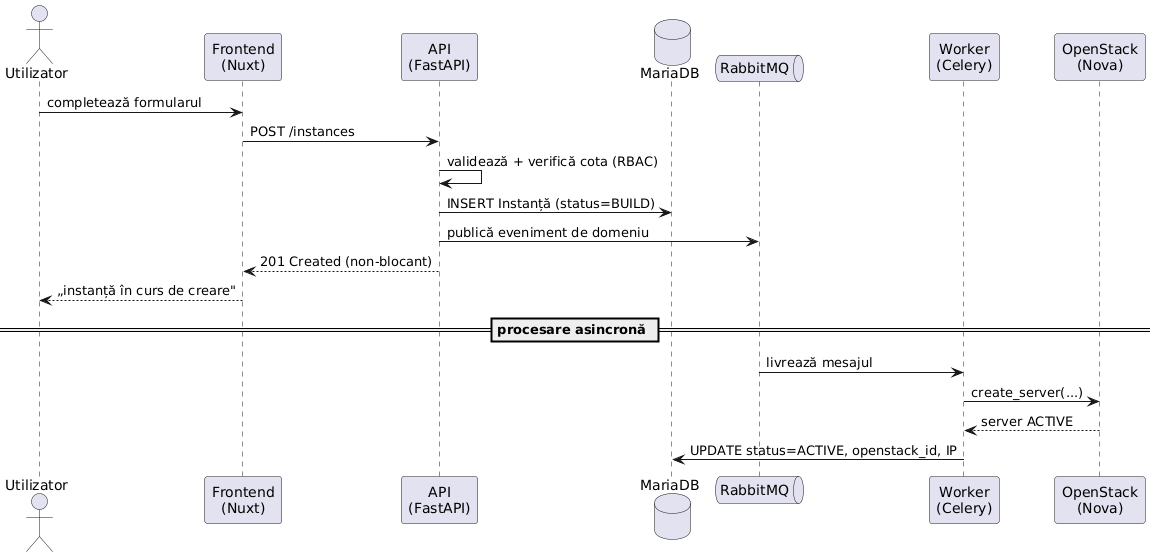
\includegraphics[width=\textwidth]{continut/capitol3/figuri/sequence.png}
    \caption{Diagrama de secvență a fluxului asincron de provizionare a unei instanțe.}
    \label{fig:secventa}
\end{figure}

Diagrama prezintă două faze separate de linia orizontală „procesare asincronă”. În \textbf{faza sincronă}, utilizatorul completează formularul în interfață, iar frontend-ul trimite o cerere \texttt{POST /instances} către API. Nivelul API validează cererea și verifică cota organizației (RBAC), inserează în MariaDB un rând de instanță cu starea inițială \texttt{BUILD}, apoi publică un eveniment de domeniu în coada RabbitMQ. Imediat după aceasta, API-ul returnează un răspuns \texttt{201 Created} neblocant, iar interfața afișează mesajul „instanță în curs de creare”. Utilizatorul nu așteaptă finalizarea operațiunii de infrastructură.

În \textbf{faza asincronă}, broker-ul livrează mesajul către un proces de fundal (\textit{worker} Celery), singurul care apelează infrastructura: acesta invocă \texttt{create\_instance} prin OpenStack SDK și așteaptă trecerea instanței în starea \texttt{ACTIVE}. La finalizare, workerul actualizează în MariaDB starea instanței (\texttt{ACTIVE}), identificatorul OpenStack și adresa IP privată, valori pe care interfața le preia la următoarea interogare periodică. Pseudocodul asociat acestui flux este prezentat în Algoritmul~\ref{alg:provisionare}.

\begin{algorithm}[H]
\caption{Provizionarea asincronă a unei instanțe}
\label{alg:provisionare}
\begin{algorithmic}[1]
\Procedure{CreareInstanta}{cerere} \Comment{sincron}
    \State validează autentificarea și permisiunile (RBAC)
    \State verifică lanțul de precondiții (cheia SSH, subrețeaua și grupul de securitate sunt provizionate)
    \State \Call{EnforceQuota}{organizație, resurse}
    \State creează rândul Instanță cu starea \texttt{BUILD} în MariaDB
    \State \textbf{commit} tranzacție
    \State \Call{Dispatch}{EvenimentProvizionareInceput}
    \State \Return 201 \Comment{răspuns neblocant}
\EndProcedure
\Statex
\Procedure{ProvisionInstance}{eveniment} \Comment{asincron}
    \State $conn \gets$ conectare la OpenStack (SDK)
    \State $server \gets$ \Call{Nova.CreateServer}{imagine, flavor, rețea, cheie, grupuri}
    \State așteaptă tranziția serverului în starea \texttt{ACTIVE}
    \If{succes}
        \State actualizează MariaDB: \texttt{openstack\_id}, \texttt{private\_ip}, starea \texttt{ACTIVE}
        \State (opțional) alocă și asociază o adresă IP flotantă
        \State (opțional) atașează volumele de stocare solicitate
    \Else
        \State marchează starea \texttt{ERROR}; reîncearcă (de cel mult 3 ori)
    \EndIf
\EndProcedure
\end{algorithmic}
\end{algorithm}

Topologia de desfășurare a infrastructurii (cluster-ul OpenStack containerizat prin Kolla-Ansible, în regim \textit{all-in-one}, accesat de la distanță prin tunelul Tailscale) este prezentată în Figura~\ref{fig:deployment}.

\begin{figure}[H]
    \centering
    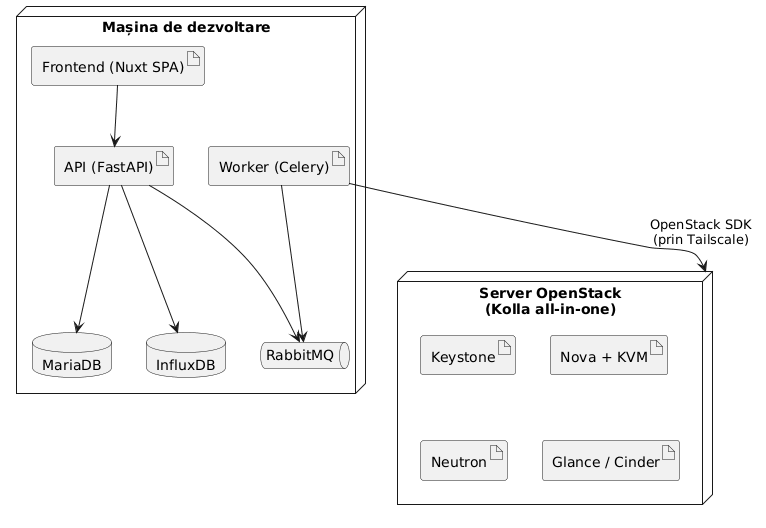
\includegraphics[width=0.85\textwidth]{continut/capitol3/figuri/deployment.png}
    \caption{Diagrama de desfășurare a mediului de testare.}
    \label{fig:deployment}
\end{figure}

Topologia separă cele două noduri ale mediului. \textbf{Mașina de dezvoltare} găzduiește întreaga stivă aplicativă: interfața (Nuxt SPA), nivelul API (FastAPI) și procesul de fundal (Celery), împreună cu serviciile de suport rulate în containere: baza de date relațională (MariaDB), baza de date de tip serii de timp (InfluxDB) și broker-ul de mesaje (RabbitMQ). Se observă că nivelul API comunică doar cu propriile baze de date și cu broker-ul, în timp ce workerul este singura componentă care comunică cu exteriorul.

\textbf{Serverul OpenStack} rulează separat, ca o mașină virtuală dedicată, pe care întregul cluster este desfășurat containerizat prin Kolla-Ansible în regim \textit{all-in-one}. Serviciile esențiale: Keystone (autentificare), Nova + KVM (calcul), Neutron (rețea) și Glance/Cinder (imagini și stocare bloc) sunt pe același nod. Singura legătură dintre cele două mașini este reprezentată de apelurile OpenStack SDK inițiate de workerul Celery, transportate prin tunelul Tailscale. Această izolare permite ca infrastructura OpenStack, cu cerințele sale ridicate de resurse, să fie găzduită independent de stiva aplicativă, reflectând totodată principiul conform căruia doar procesele de fundal interacționează cu infrastructura.

\subsection{Scalabilitate și concurență}
\label{subsec:cap3_scalabilitate}

Decuplarea prin brokerul de mesaje oferă arhitecturii o proprietate esențială: nivelul API și procesele de fundal pot fi scalate independent. Întrucât serverul web nu execută niciodată operațiunile costisitoare, ci doar le publică în coadă, capacitatea de procesare a infrastructurii poate fi mărită prin simpla adăugare de noi workeri Celery, fără a modifica sau a multiplica serverul API. Pe un sistem de producție Linux, fiecare worker rulează cu un \textit{pool} de procese, executând mai multe sarcini în paralel; numărul total de sarcini concurente este astfel produsul dintre numărul de workeri și dimensiunea \textit{pool}-ului, ajustabil în funcție de încărcare.

 Deoarece starea de sesiune este păstrată doar în token-uri JWT, nu pe server, nivelul API este \textit{stateless} și poate fi, la rândul său, replicat în spatele unui distribuitor de sarcină (\textit{load balancer}). Singura limitare a configurației de dezvoltare este rularea workerului pe Windows cu opțiunea \texttt{--pool=solo}, care serializează execuția sarcinilor; aceasta nu reflectă o constrângere a arhitecturii, ci a mediului, fiind eliminată utilizând Linux.

\subsection{Reconcilierea stării și rezolvarea conflictelor}
\label{subsec:cap3_reconciliere}

Întrucât resursele pot fi modificate și în afara platformei --- de exemplu, direct din interfața nativă OpenStack (Horizon) sau în urma unei defecțiuni a unei mașini virtuale --- starea memorată în baza de date se poate desincroniza de starea reală a infrastructurii. Pentru a corecta automat aceste divergențe, o sarcină periodică de reconciliere (\texttt{sync\_instance\_states}), rulată de Celery Beat la fiecare 30 de secunde, compară starea fiecărei instanțe cu cea raportată de Nova și o aliniază, conform Algoritmului~\ref{alg:reconciliere}.

\begin{algorithm}[H]
\caption{Reconcilierea periodică a stării instanțelor}
\label{alg:reconciliere}
\begin{algorithmic}[1]
\Procedure{SyncInstanceStates}{} \Comment{rulat de Celery Beat la fiecare 30 s}
    \State conectare la OpenStack (SDK)
    \State \textit{vii} $\gets$ tabela (\texttt{openstack\_id} $\rightarrow$ stare) a tuturor serverelor raportate de Nova
    \ForAll{instanța $i$ din baza de date cu \texttt{openstack\_id} nenul}
        \If{starea lui $i$ este tranzitorie} \Comment{BUILD, DELETING, STOPPING, STARTING, REBOOT}
            \State treci la următoarea instanță \Comment{operațiune locală în curs --- nu se suprascrie}
        \EndIf
        \State \textit{stareReală} $\gets$ starea din \textit{vii} corespunzătoare lui $i$, sau \texttt{ERROR} dacă identificatorul nu apare
        \If{\textit{stareReală} diferă de starea curentă a lui $i$}
            \State înregistrează tranziția în jurnalul de evenimente al instanței
            \State actualizează starea lui $i$ la valoarea reală \Comment{OpenStack = sursă de adevăr}
        \EndIf
    \EndFor
    \State \textbf{commit} tranzacție
\EndProcedure
\end{algorithmic}
\end{algorithm}

Logica de rezolvare a conflictelor pornește de la principiul că, pentru stările stabile, \textbf{OpenStack constituie sursa de adevăr}. Excepția esențială o reprezintă instanțele aflate într-o stare tranzitorie (creare, ștergere, pornire, oprire sau repornire în curs), care sunt ignorate de reconciliere, astfel încât o operațiune locală în desfășurare să nu fie suprascrisă de un instantaneu intermediar al infrastructurii. O stare de eroare nu este definitivă: dacă serverul redevine activ, trecerea următoare readuce instanța în starea \texttt{ACTIVE}.

Ștergerea manuală a unei mașini dintr-o interfață externă este tratată printr-o valoare implicită: dacă identificatorul instanței nu mai apare în lista serverelor Nova, reconcilierea îi atribuie starea \texttt{ERROR} și consemnează evenimentul în jurnal. Astfel, instanța nu dispare silențios, ci este semnalată în interfață, de unde poate fi eliminată definitiv --- moment în care, serverul nemaiexistând în OpenStack, se șterge doar rândul corespunzător din baza de date. Adresele IP flotante urmează un tratament fidel modelului \textit{Elastic IP} din AWS: la ștergerea unei instanțe, adresa este \textit{disociată} (revine în bazinul rezervat al organizației, reutilizabilă), nu eliberată; reconcilierea unei adrese rămase orfane în urma unei ștergeri externe are loc la eliminarea instanței prin platformă, o curățare periodică dedicată a acestora constituind o posibilă direcție de dezvoltare ulterioară.

\section{Paradigme de programare utilizate}
\label{sec:cap3_tipare}

Mentenabilitatea codului backend a fost asigurată prin adoptarea unor paradigme de programare care structurează interacțiunea cu baza de date și comunicarea cu procesele de fundal.

\begin{itemize}
    \item \textbf{Paradigma Repository:} Fiecare entitate dispune de un depozit (\textit{repository}) specializat, care expune operațiile de acces la date și încapsulează interogările specifice domeniului (de regulă filtrate după organizație). Astfel, logica de business nu construiește direct interogări SQL.
    \item \textbf{Paradigma Unit of Work:} Toate depozitele sunt grupate sub o singură sesiune de bază de date. Un serviciu primește o unitate de lucru (\textit{Unit of Work}), poate opera asupra mai multor depozite și confirmă tranzacția (\textit{commit}) o singură dată, garantând atomicitatea.
    \item \textbf{Domain Events:} Serviciile emit evenimente sub formă de obiecte simple de date, iar un dispecer le rutează către gestionarii înregistrați. Acest tipar permite ca logica de business să rămână complet independentă de tehnologia de procesare asincronă.
\end{itemize}

Relațiile dintre serviciu, unitatea de lucru, depozite și mecanismul de evenimente sunt ilustrate în diagrama de clase prezentată în Anexa~\ref{anexa:class}. Cele trei tipare funcționează în jurul clasei centrale \texttt{Service}: aceasta \textit{folosește} o instanță \texttt{UnitOfWork}, care la rândul ei \textit{agregă} depozitele specializate (\texttt{Repository}) sub o singură sesiune și expune metoda \texttt{commit()}. Pentru comunicarea cu infrastructura, serviciul nu apelează direct procesele de fundal, ci creează un obiect \texttt{DomainEvent} și îl transmite metodei \texttt{dispatch(event)} a clasei \texttt{Dispatcher}, care rutează evenimentul către gestionarul (\textit{handler}) înregistrat prin \texttt{on(EventType)}; acesta declanșează în final sarcina asincronă prin \texttt{.delay()}. Se evidențiază astfel decuplarea esențială: clasa \texttt{Service} depinde doar de abstracțiuni (unitatea de lucru și dispecerul) și nu are nicio referință directă către Celery.

\section{Proiectarea bazei de date}
\label{sec:cap3_baza_date}

Baza de date relațională a fost proiectată respectând forma normală 3 (3NF). Interacțiunea cu MariaDB se realizează prin intermediul ORM-ului (\textit{Object-Relational Mapping}) SQLAlchemy, care previne vulnerabilitățile de tip SQL Injection și permite interogări asincrone.

Baza de date stochează local metadatele resurselor OpenStack (identificatorii \texttt{openstack\_id} returnați de Nova sau Neutron). Astfel, nivelul API poate răspunde instantaneu la cererile de citire, fără a interoga infrastructura. Pachetele hardware (\textit{flavors}) nu sunt stocate într-un tabel, ci sunt definite static în cod (corespunzând celor existente în OpenStack) pentru a evita o sincronizare suplimentară.

Schema relațională este compusă din următoarele entități principale:

\begin{itemize}
    \item \textbf{\texttt{Organization}:} Unitatea de izolare (\textit{tenant}). Toate resursele sunt asociate unei organizații, ceea ce stă la baza modelului multi-tenant.
    \item \textbf{\texttt{User}:} Identitatea unui utilizator (\texttt{email}, \texttt{role}, \texttt{is\_active}). Parolele sunt stocate exclusiv ca amprente criptografice (\textit{bcrypt}), iar amprenta token-ului de reîmprospătare (\texttt{refresh\_token\_hash}) permite revocarea sesiunii.
    \item \textbf{\texttt{Instance}:} Resursa centrală. Reține organizația și utilizatorul proprietar, cheia SSH, subrețeaua, identificatorul \texttt{openstack\_id}, adresa IP privată (\texttt{private\_ip\_address}) și starea de execuție (\texttt{status}).
    \item \textbf{\texttt{Keypair}:} Cheile SSH publice încărcate sau generate de utilizatori, injectate de Nova în mașini la instanțiere.
    \item \textbf{\texttt{Network} și \texttt{Subnet}:} Rețelele private și subrețelele organizației, împreună cu identificatorii lor OpenStack (\texttt{openstack\_network\_id}, \texttt{openstack\_router\_id}).
    \item \textbf{\texttt{SecurityGroup}} (și regulile asociate): Grupuri de securitate reutilizabile, legate de instanțe printr-o relație multi-la-multi.
    \item \textbf{\texttt{FloatingIP}:} Adresele IP publice ca resurse de sine stătătoare, cu o legătură opțională către o instanță (\textit{SET NULL} la ștergere).
    \item \textbf{\texttt{Volume}:} Volumele de stocare bloc (Cinder), org-scoped, cu o legătură opțională către instanța la care sunt atașate.
    \item \textbf{\texttt{Image}:} Imaginile de sistem personalizate (importate de la URL sau rezultate din \textit{snapshot}-uri), cu indicator de vizibilitate publică/privată.
    \item \textbf{\texttt{Quota}:} Limitele de resurse configurabile per organizație.
    \item \textbf{\texttt{InstanceEvent}:} Jurnalul de evenimente al fiecărei instanțe (severitate, mesaj, marcaj temporal), șters în cascadă odată cu instanța.
\end{itemize}

Relațiile dintre aceste tabele sunt ilustrate în diagrama Entity-Relationship (ER), prezentată în Anexa~\ref{anexa:er}.

\section{Securitatea și controlul accesului}
\label{sec:cap3_securitate}

Securitatea platformei este împărțită în: autentificarea, autorizarea și izolarea datelor.

\textbf{Autentificarea} este realizată prin token-uri JWT (\textit{JSON Web Tokens}) păstrate în cookie-uri de tip \textit{httpOnly}, inaccesibile codului JavaScript, ce nu permite atacurile de tip XSS asupra sesiunii. Modelul folosește un token de acces cu durată scurtă de viață și un refresh token cu durată lungă; la expirarea token-ului de acces, aplicația client solicită un token nou. Amprenta refresh token-ului este stocată pe rândul utilizatorului, ce permite revocarea sesiunii la deconectare. Fluxul de autentificare și reîmprospătare este prezentat în Figura~\ref{fig:auth_flow}.

\begin{figure}[H]
    \centering
    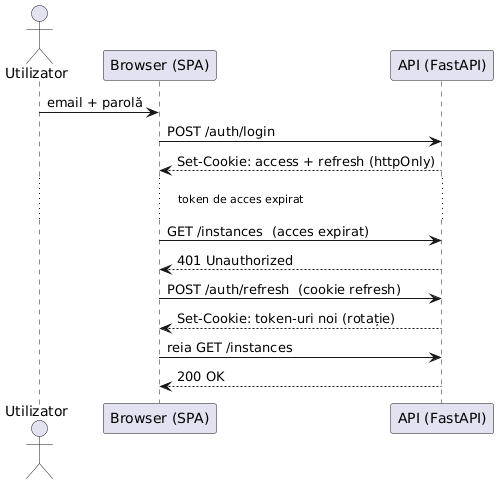
\includegraphics[width=0.7\textwidth]{continut/capitol3/figuri/auth_flow.png}    
    \caption{Diagrama de secvență a fluxului de autentificare.}
    \label{fig:auth_flow}
\end{figure}

Diagrama ilustrează mecanismul de refresh a sesiunii. La autentificare, utilizatorul transmite email-ul și parola, iar în urma cererii \texttt{POST /auth/login} serverul setează două cookie-uri \textit{httpOnly}: token-ul de acces (de scurtă durată) și cel de refresh (de lungă durată). Atunci când token-ul de acces expiră, o cerere ulterioară este respinsă cu \texttt{401 Unauthorized}. Aplicația client interceptează automat acest răspuns și emite o cerere \texttt{POST /auth/refresh}, însoțită de cookie-ul de refresh; serverul validează amprenta stocată, emite o nouă pereche de token-uri (\textit{rotație}) și o setează din nou ca \textit{cookie}. În final, clientul reia cererea inițială, care de această dată are succes (\texttt{200 OK}). Tot procesul se desfășoară fără intervenția utilizatorului și fără ca scriptul JavaScript să acceseze vreodată token-urile, acestea fiind protejate în cookie-uri inaccesibile codului din pagină.

\textbf{Autorizarea} se bazează pe un model de roluri (\textit{Role-Based Access Control}), centralizat într-o singură politică de permisiuni. Rolurile de proprietar și membru sunt specifice organizației, în timp ce rolul de administrator operează la nivelul întregii platforme. Operațiunile distructive (ștergerea instanțelor, eliberarea adreselor IP) sunt destinate proprietarului, iar accesul la zona de administrare este protejat separat.

\textbf{Izolarea datelor} este asigurată la nivelul aplicației: fiecare interogare este filtrată după identificatorul organizației, astfel încât un utilizator nu poate accesa resursele altei organizații. Această decizie de proiectare (toate organizațiile partajează un singur proiect OpenStack, izolarea fiind logică, nu la nivel de infrastructură) este analizată din perspectiva limitărilor în capitolul de testare.

\section{Descrierea implementării soluției}
\label{sec:cap3_implementare}

Implementarea concretizează arhitectura descrisă anterior. Procesul de provizionare a unei instanțe începe prin recepționarea unei cereri HTTP la nivelul API. Cererea este supusă unui mecanism de validare structurală și semantică (prin Pydantic), care verifică inclusiv lanțul de precondiții: cheia SSH, subrețeaua și grupul de securitate trebuie să fie deja provizionate în OpenStack (identificatorii lor \texttt{openstack\_id} să fie completați). În caz contrar, cererea este respinsă imediat cu un cod de eroare corespunzător.

După validare și verificarea cotei organizației, logica aplicației inițiază o tranzacție în MariaDB, creând una sau mai multe entități Instance cu starea \texttt{BUILD}, după care emite câte un eveniment de domeniu pentru fiecare. Deoarece evenimentele sunt rutate către gestionari care publică mesaje în RabbitMQ, serverul web returnează imediat un răspuns de succes, eliberând firul de execuție.

Ulterior, procesul de fundal Celery extrage mesajul și declanșează secvența de interacțiune cu OpenStack: identifică imaginea, pachetul hardware (flavour) și cheia, rezolvă rețeaua pornind de la subrețea, creează serverul prin Nova și așteaptă tranziția în starea \texttt{ACTIVE}. La finalizare, actualizează baza de date cu identificatorul OpenStack și adresa IP privată și, opțional, alocă o adresă IP publică și atașează volumele solicitate. Eventualele eșecuri sunt tratate prin reluarea automată a sarcinii, iar starea instanței este marcată \texttt{ERROR} dacă reîncercările nu reușesc.

Pentru a menține concordanța dintre starea afișată și starea reală a infrastructurii, un proces periodic (\textit{Celery Beat}) reconciliază la intervale regulate stările instanțelor cu starea raportată de Nova, reflectând astfel și modificările apărute în afara platformei. Tot un proces periodic colectează telemetria de performanță a instanțelor, mecanism detaliat în Secțiunea~\ref{sec:cap3_telemetrie}.

Suportul pentru \textit{Cloud-init} este integrat nativ în acest flux: un script de inițializare furnizat de utilizator (sau asociat unui șablon preconfigurat) este transmis instanței prin serviciul de metadate al Nova și executat la prima pornire, permițând configurarea automată a mașinii fără intervenție prin SSH.

\section{Telemetria și monitorizarea performanței}
\label{sec:cap3_telemetrie}

Monitorizarea consumului de resurse al mașinilor virtuale ridică o problemă de proiectare distinctă față de gestiunea stării: în timp ce datele tranzacționale (utilizatori, instanțe, rețele) se pretează unei baze de date relaționale, metricile de performanță (consum de procesor și memorie) sunt date secvențiale, generate continuu și marcate temporal (\textit{timestamps}), al căror volum ar degrada rapid performanța unui sistem relațional. Din acest motiv, platforma adoptă o \textbf{persistență hibridă}: datele de stare rămân în MariaDB, iar telemetria este stocată separat într-o bază de date de tip \textit{Time-Series}, InfluxDB, optimizată nativ pentru ingestia rapidă a metricilor și pentru agregarea lor pe intervale de timp.

Lanțul de telemetrie respectă aceeași separare a responsabilităților ca restul sistemului. Un proces periodic \textit{Celery Beat} declanșează, la interval fix, o sarcină de colectare care, pentru fiecare instanță activă, interoghează diagnosticele de performanță expuse de Nova prin SDK, apelul către infrastructură rămânând exclusiv în procesul de fundal. Metricile obținute sunt scrise ca puncte în InfluxDB, etichetate cu identificatorul instanței. La cerere, API-ul FastAPI \textbf{doar citește} seria temporală corespunzătoare unei instanțe și o returnează interfeței, care o interoghează periodic și o redă sub forma unui grafic în pagina de detaliu. Întrucât graficul este reconstituit din InfluxDB la fiecare încărcare, istoricul de consum este persistent și supraviețuiește reîmprospătării paginii. Rezultatul vizual al acestui mecanism este prezentat în Capitolul~\ref{cap:cap4}, în cadrul validării.

\section{Interfața cu utilizatorul}
\label{sec:cap3_interfata}

Interfața grafică a fost proiectată după principiul ascunderii complexității, oferind fluxuri de lucru simple pentru sarcinile uzuale. Tabloul de bord (\textit{dashboard}) prezintă lista instanțelor cu stările lor actualizate periodic, pagina de creare ghidează utilizatorul prin selecția imaginii, a pachetului hardware și a opțiunilor de rețea și stocare, iar pagina de detaliu a instanței centralizează specificațiile, conexiunea SSH, consola, jurnalele și graficul de consum. O zonă distinctă, accesibilă doar administratorului, oferă o vedere de ansamblu asupra întregii platforme.

Capturi de ecran reprezentative ale acestor pagini, surprinse din aplicația în funcțiune, sunt prezentate în Capitolul~\ref{cap:cap4}, dedicat testării și rezultatelor.

\subsection{Arhitectura aplicației client}
\label{subsec:cap3_frontend}

Interfața este o aplicație de tip \textit{Single-Page Application} (SPA), generată integral pe partea de client (\textit{Server-Side Rendering} dezactivat). Această alegere este motivată de două considerente: pe de o parte, aplicația este un panou de administrare destinat utilizatorilor autentificați, pentru care indexarea de către motoarele de căutare este irelevantă; pe de altă parte, și mai important, generarea pe partea de client simplifică gestiunea sesiunii bazate pe cookie-uri \textit{httpOnly}. Întrucât autentificarea se realizează prin astfel de cookie-uri, codul JavaScript nu are niciodată acces la token-ul JWT, nu îl stochează și nu îl citește, ci își deduce starea de autentificare interogând endpoint-ul \texttt{/auth/me}.

Starea aplicației este gestionată centralizat printr-o bibliotecă de tip \textit{store} (Pinia). Un depozit de sesiune constituie unicul punct de referință pentru utilizatorul autentificat, rolul său și permisiunile derivate, expunând proprietăți calculate (precum \textit{is authenticated}, \textit{is owner}, \textit{is admin}) pe baza cărora interfața ascunde acțiunile pe care un rol nu le poate efectua. Token-ul nu face parte din starea acestui depozit, el rămâne exclusiv în cookie. În schimb, datele specifice fiecărei pagini (lista instanțelor, a volumelor etc.) sunt încărcate prin mecanismul nativ al meta-framework-ului, cu interogare periodică (\textit{polling}), păstrând astfel actualizarea în timp real a stărilor afișate.

Cel mai important mecanism al stratului client este tratarea transparentă a sesiunii. Toate apelurile către API sunt centralizate într-o singură funcție de abstractizare, care transmite cookie-urile la fiecare cerere. La expirarea token-ului de acces (cu durată scurtă de viață), o cerere primește răspunsul \texttt{401}; în acest moment, funcția apelează automat endpoint-ul de refresh, cu deduplicare de tip \textit{single-flight}, astfel încât mai multe cereri concurente eșuate declanșează un singur refresh, după care reia cererea inițială, fără ca utilizatorul să observe vreo întrerupere. Un \textit{middleware} global rezolvă sesiunea la fiecare schimbare de rută, iar un proces de tip \textit{watcher} redirecționează către pagina de autentificare dacă sesiunea expiră în timpul utilizării. Împreună, aceste mecanisme ascund complet ciclul de viață al token-ului de acces, oferind o experiență fluidă și securizată utilizatorului.